
\documentclass{beamer}
\usetheme{Madrid}
\usepackage{amsmath,amsthm,amsfonts,amssymb}
\usepackage{graphicx}
\usepackage{hyperref}
\usepackage{enumerate}
\usepackage[style=authoryear, maxcitenames=1, dashed=false]{biblatex}
\addbibresource{citations.bib}


\DeclareMathOperator*{\argmin}{arg\,min}

\newcommand{\R}{\mathbb{R}}
\newcommand{\Borel}[1]{\mathcal{B}\paren{#1}}
\newcommand{\0}{\emptyset}
\newcommand{\prob}{\mathbb{P}}
\newcommand{\E}{\mathbb{E}}
\newcommand{\Ep}[1]{\mathbb{E}\left[ #1 \right]}
\newcommand{\paren}[1]{\left(#1 \right)}
\newcommand{\sqbr}[1]{\left[#1 \right]}
\newcommand{\set}[1]{\left\{ #1 \right\}}
\newcommand{\norm}[1]{|\hspace{-1pt}|#1 |\hspace{-1pt}|}
\newcommand{\normsq}[1]{\norm{#1}^{2}}
\newcommand{\ind}[1]{\mathmybb{1}_{\sqbr{#1}}}
\newcommand{\data}{\mathcal{D}_{n}}
\newcommand{\Hcal}{\mathcal{H}}
\newcommand{\Acal}{\mathcal{A}_{n}}
\newcommand{\Tcal}{\mathcal{T}_{n}}
\newcommand{\Ncal}{\mathcal{N}}
\newcommand{\Mcal}{\mathcal{M}}
\newcommand{\Fcal}{\mathcal{F}}
\newcommand{\aseq}{\stackrel{\mathrm{a.s.}}{=}}
\newcommand{\X}{\boldsymbol{X}}
\newcommand{\x}{\boldsymbol{x}}
\newcommand{\z}{\boldsymbol{z}}
\newcommand{\y}{\boldsymbol{y}}
\newcommand{\e}{\boldsymbol{e}}
\newcommand{\Cov}[1]{\mathrm{Cov}\paren{#1}}
\newcommand{\bbeta}{\boldsymbol{\beta}}
\newcommand{\bbetahat}{\boldsymbol{\hat{\beta}}}
\newcommand{\bepsilon}{\boldsymbol{\epsilon}}
\newcommand{\Loss}[1]{L_{n}\paren{#1}}
\newcommand{\Rhat}[2]{\hat{R}_{n, #1}\paren{#2}}
\newcommand{\alphahat}[1]{\hat{\alpha}^{#1}}
\newcommand{\alphatilde}{\tilde{\alpha}}
\newcommand{\alphabar}{\bar{\alpha}}
\newcommand{\lev}{h_{ii,\alpha}}
\newcommand{\loocv}[1]{\hat{R}^{(1)}_{n}\paren{#1}}
\newcommand{\ho}{\hat{R}_{\mathrm{ho}}}
\newcommand{\op}[1]{o_{\prob}\paren{#1}}
\newcommand{\Op}[1]{O_{\prob}\paren{#1}}
\newcommand{\sigmahat}{\hat{\sigma}^{2}_{n}}
\newcommand{\fhat}[2]{\hat{f}_{#1, #2}}
\newcommand{\ftilde}[1]{\tilde{f}_{#1}}
\newcommand{\lambdahat}[1]{\hat{\lambda}_{#1}}
\newcommand{\blambdahat}{\boldsymbol{\hat{\lambda}}}
\newcommand{\pen}[1]{\mathrm{pen}\paren{#1}}
\newcommand{\penBIC}[1]{\mathrm{pen}_{\mathrm{BIC}}\paren{#1}}
\newcommand{\tr}[1]{\mathrm{tr}\paren{#1}}
\newcommand{\ols}[1]{\paren{\X^{\top}_{#1}\X_{#1}}\X^{\top}_{#1}\y}
\newcommand{\fho}{\hat{f}^{(\mathrm{ho})}_{n}}

% For indicator functions:
\DeclareMathAlphabet{\mathmybb}{U}{bbold}{m}{n}
\newcommand{\1}{\mathmybb{1}}

\title[CV for Selection]{MATH 410 Project: The Asymptotics of Cross-Validation for Model Selection in the Regression Setting}
\author[Diego Urdapilleta]{Diego Urdapilleta de la Parra}
\subtitle{Supervised by: Prof.\ Mehdi Dagdoug}
\institute[McGill]{McGill University}
\date{2025}

\AtBeginSection[]
{
  \begin{frame}
    \frametitle{Table of Contents}
    \tableofcontents[currentsection]
  \end{frame}
}

\begin{document}

\begin{frame}
  \titlepage{}
\end{frame}

\section{Introduction}
\begin{frame}{The problem of model selection}

    \textbf{Setting: } Multiple competing candidate models for a regression task.

    \textbf{Some considerations:}
    \begin{itemize}
        \item Striking a balance: Simpler models offer efficiency and stability, but may underfit; complex models capture structure, but risk overfitting.

        \item Theoretical assumptions behind models are often unverifiable, motivating comparisons among alternatives.
    \end{itemize}

    This work explores the asymptotic behavior of cross-validation as a model selection critetion.
\end{frame}

\begin{frame}{Outline}
    \tableofcontents
  \end{frame}

\begin{frame}{Setup and Notation}
    For positive integers $n$ and $p_{n}$, let $(y, \x):\Omega\to\R\times{[0,1]}^{p_{n}}$ be a real-valued random vector with distribution $\mu_{y, \x}$ such that 
    \begin{itemize}
        \item $\E{|y|^{2}}<\infty$
        \item $\E\normsq{\x}<\infty$
        \item $\Ep{\x\x^{\top}}\succ 0$
    \end{itemize}

    A Borel-measurable function \(f:{[0,1]}^{p_{n}} \to \R\) that satisfies
    \[f(\x) \aseq \Ep{y\mid \x}\]
    is called the \emph{regression} function of \(y\) on \(\x\). 
  
    Let \(\data := \set{\paren{y_{i}, \x_{i}}:i\in [n]}\) be a sample of independent data points drawn from \(\mu_{y, \x}\).
    Define the residual \(\epsilon_{i}:= y_{i} - f(\x_{i})\), which yields the decomposition
  \[y_{i} = f(\x_{i}) + \epsilon_{i}, \quad i\in[n],\]
\end{frame}

\begin{frame}{Cross-validation}  
    Let \(J\) be an index set and let \(\set{E_{j}}_{j\in J}\) be a family of subsets \(E_{j}\subset [n]\) such that \(|E_{j}|=n_{1}\) for all \(j\in J\), and write \(V_{j} := E_{j}^{c}\). 
  
    For each subset \(E_{j}\), we consider the estimation sample \(\data^{E_{j}}\) of \(n_{1}\) data ponts given by
    \[\data^{E_{j}} = \set{\paren{y_{i}, \x_{i}}\in\data :i\in E_{j}}.\]

    For each \(j\in J\), we fit the model \(\hat{f}\) on the estimation sample \(\data^{E_{j}}\) and compute the \alert{\emph{hold-out}} loss against the remaining \(n-n_{1}=: n_{2}\) data points in \(\data^{V_{j}}\):
    \[\hat{R}_{n}^{E_{j}} := \frac{1}{n_{2}}\sum_{i \in V_{j}} \paren{y_{i} - \hat{f}\paren{\x_{i};\data^{E_{j}}}}^{2}\]
\end{frame}

\begin{frame}{Cross-validation}
    The cross-validation loss estimator is
    \[\hat{R}^{CV}_{n}:= \frac{1}{|J|}\sum_{j\in J}\hat{R}_{n}^{E_{j}}.\]

    Different choices of  \(J\) and estimation size \(n_{1}\) yield different variants of cross-validation.
  
    Examples:
    \begin{itemize}
        \item \(n_{1}=n-1\) for the \emph{leave-one-out} estimator,
        \item \(|J|=k\) and \(n_{1} = n(k-1)/k\) for the \emph{\(k\)-fold} estimator.
    \end{itemize}

\end{frame}

\section{Variable Selection for Linear Models}\label{sec:lm}

\begin{frame}{Linear models: Setup}
    
    We let \(\Acal\subset2^{[p_{n}]}\) be a family of index sets representing candidate models. For \(\alpha\in\Acal\), we write by \(p_{n}(\alpha) := |\alpha|\) and consider
    \[f_{\alpha}(\X) = \X_{\alpha}\bbeta_{\alpha},\]

    \begin{enumerate}
        \item We say \(\alpha\in\Acal\) is \emph{correct} if \(\X\bbeta\aseq f_{\alpha}(\X)\), and we denote by \(\Tcal\) the set of correct models in \(\Acal\).
        \item We say \(\alpha\in\Acal\) is \emph{wrong} if it is not correct, and we denote by \(\Tcal^{c}\) the set of wrong models in \(\Acal\).
        \item We say \(\Acal\) is \emph{embedded} if there exists an enumeration \(\alpha_{1}, \alpha_{2}, \ldots, \alpha_{k}\) of all elements in \(\Acal\) such that \[\alpha_{1}\subset\alpha_{2}\subset\cdots\subset\alpha_{k}.\]
    \end{enumerate}

\end{frame}

\begin{frame}{Linear models: Setup}
    \begin{example}
        Suppose that we have the underlying model \(\Ep{y\mid\x} \aseq \X\bbeta\) given by
        \[\X = \begin{bmatrix}
          | & | & | & |\\
          \x^{(1)} & \x^{(2)} & \x^{(3)} & \x^{(4)} \\
          | & | & | & |
        \end{bmatrix}\quad\text{and}\quad \bbeta = \begin{bmatrix}
          2\\
          5\\
          3\\
          0
        \end{bmatrix}\]
        We consider \(\Acal = \set{\alpha_{1}, \alpha_{2}, \alpha_{3}}\) with
        \begin{align*}
            \alpha_{1} = \set{1,2},\quad\alpha_{2}=\set{1,2,3},\quad\text{and}\quad\alpha_{3} = \set{1,2,3,4}
        \end{align*}
        The model \(\alpha_{2}\) is correct:
        \[\X_{\alpha_{2}}\bbeta_{\alpha_{2}} = \begin{bmatrix}
          | & | & | \\
          \x^{(1)} & \x^{(2)} & \x^{(3)} \\
          | & | & | 
        \end{bmatrix}\begin{bmatrix}
          2\\
          5\\
          3
        \end{bmatrix} = \X\bbeta\]
      
    \end{example}

\end{frame}

\begin{frame}
    \frametitle{Linear models: Consistency and efficiency}
    Define the losses
    \[\Loss{\alpha}:=\frac{1}{n}\normsq{f(\X) - \hat{f}_{\alpha}\paren{\X}}\quad\text{and}\quad R_{n}(\alpha):= \Ep{\Loss{\alpha}\mid\X}\]
    for \(\alpha\in\Acal\), with \(\hat{f}_{\alpha}(\X):=\X_{\alpha}\bbetahat_{\alpha}\).

    Let \(\hat{R}_{n}\) be a model selection criterion and let \(\alphahat{}_{n}\) be the model selected by minimizing \(\hat{R}_{n}\) over \(\Acal\). Let \(\alpha^{*}_{n}\) denote the model minimizing \(R_{n}\) over \(\Acal\). We say that \(\hat{R}_{n}\) is \alert{consistent} if 
    \[\prob\set{\alphahat{}_{n} = \alpha^{*}_{n}}\to 1\]
    as \(n\to\infty\). We say that \(\hat{R}_{n}\) is \alert{assymptotically loss efficient} if 
    \[\frac{L_{n}(\alphahat{}_{n})}{L_{n}(\alpha^{*}_{n})}\xrightarrow{\prob} 1.\]
  
\end{frame}

\begin{frame}{The leave-one-out}
    We define the leave-one-out loss estimator for a model \(\alpha\in\Acal\) to be 
    \[\loocv{\alpha} := \frac{1}{n}\sum_{i=1}^{n}\paren{(y_{i} - \x_{i\alpha}^{\top}\bbetahat_{\alpha}^{(i)})}.\]

    \begin{block}{Proposition}
        For \(\alpha\in\Acal\), the leave-one-out estimator \(\loocv{\alpha}\) satisfies the following equality:
        \[\loocv{\alpha}= \frac{1}{n}\sum_{i=1}^{n}\paren{\frac{y_{i}-\x_{i\alpha}^{\top}\bbetahat_{\alpha}}{1-h_{ii,\alpha}}}^{2},\]
        where \(h_{ii,\alpha} = \x_{i\alpha}^{\top}{(\X_{\alpha}^{\top}\X_{\alpha})}^{-1}\x_{i\alpha}\) denotes the \(i\)th leverage and \(\bbetahat_{\alpha}\) is the OLS estimator for model \(\alpha\) fitted on the whole data set.
    \end{block}
\end{frame}

\begin{frame}{The leave-one-out}
    \begin{block}{Proposition (\cite{shao_1993})}
        Suppose that \(\Tcal\) is non-empty and let \(\alphahat{(1)}\) be the model minimizing \(\loocv{\alpha}\).
            \begin{enumerate}
                \item Under H1, H2, and H3, \[\lim_{n\to\infty}\prob\set{\alphahat{(1)}\in\Tcal^{c}}=0.\]
                \item If \(p(\alpha^*) < p\), \[\lim_{n\to\infty}\prob\set{\alphahat{(1)}=\alpha^{*}}\neq 1.\]
            \end{enumerate}
    \end{block}
\end{frame}

\begin{frame}{The leave-one-out}
    \textbf{Interpretation: } The leave-one-out places too much weight on the estimation and too little on the evaluation.
    \begin{itemize}
        \item \(R_{n_{1}}(\alpha) = \sigma^{2}p(\alpha)/n_{1}\) for \(\alpha\in\Tcal\).
        \item The larger \(n_{1}\), the closer \(R_{n_{1}}(\alpha)\) is to a flat line.
        \item The leave-one-out, adopts the largest possible \(n_{1}= n-1\), making it difficult for the estimator to distinguish between correct models.
      \end{itemize}  

    \textbf{Conjecture: } A smaller estimation set and a larger validation set might improve the performance of cross-validation procedures for model selection.
\end{frame}

\begin{frame}{A general perspective: the GIC}
  
    A large portion of selection criteria in the literature can be reduced to a general penalized criterion with a penalty of the type 
    \[\mathrm{pen}_{\lambda_{n}}(\alpha) = \frac{1}{n} \lambda_{n} \sigmahat p_{n}(\alpha),\]
    for some some estimator \(\sigmahat\) of \(\sigma^{2}\) and a sequence of real numbers \(\set{\lambda_{n}}_{n\geq 1}\) satisfying \(\lambda_{n}\geq 2\) and \(\lambda_{n}/n\to 0\). This penalty yields the \alert{\emph{Generalized Information Criterion}}~(\cite{shao_1997}):
    \[\Rhat{\lambda_{n}}{\alpha} := \frac{1}{n}\normsq{\y - \X_{\alpha}\bbetahat_{\alpha}} + \frac{1}{n}\lambda_{n}\sigmahat p_{n}(\alpha)\quad\text{for }\alpha\in\Acal,\]

    We consider two cases: \(\lambda_{n}\equiv 2\) and \(\lambda_{n}\to\infty\)
\end{frame}

\begin{frame}{GIC:\@ The case of \(\lambda_{n} \equiv 2\)}
  
\begin{block}{Theorem}
    Suppose that \(\sigmahat\) is consistent for \(\sigma^{2}\). Under some regularity assumptions, 
    \begin{enumerate}
        \item If \(|\Tcal|\leq1\) for all but finitely many \(n\), then \(\hat{R}_{n,2}\) is asymptotically loss efficient.
        \item Suppose that \(|\Tcal|> 1\) for all but finitely many \(n\). If there exists a positive integer \(m\) such that \(\Ep{y_{1} - \x_{1}^{\top}\bbeta}^{4m}<\infty\) and 
        \begin{equation}\label{eq:conditionsums}
            \sum_{\alpha\in\Tcal}\frac{1}{\paren{p_{n}(\alpha)}^{m}}\xrightarrow{n\to\infty} 0 \quad\text{or}\quad \sum_{\substack{\alpha\in\Tcal,\\ \alpha\neq\alpha^{*}}}\frac{1}{\paren{p_{n}(\alpha) - p_{n}(\alpha^{*})}^{m}}\xrightarrow{n\to\infty} 0,
        \end{equation}
        then \(\hat{R}_{n,2}\) is asymptotically loss efficient.
    \end{enumerate}
\end{block}
\end{frame}

\begin{frame}{GIC:\@ The case of \(\lambda_{n} \equiv 2\)}
    \begin{block}{Theorem (continued)}
        \begin{itemize}
            \item Suppose that \(|\Tcal|>1\) for all but finitely many \(n\). 
            If \(|\Tcal|\) is bounded,
            then the condition that
            \begin{equation}
                \label{eq:conditionP}
                p_{n}(\alpha^{*}_{n})\to\infty\quad\text{or}\quad \min_{\substack{\alpha\in\Tcal,\\ \alpha\neq\alpha^{*}}}\paren{p_{n}(\alpha) - p_{n}(\alpha^{*})}\to\infty
            \end{equation}
            is necessary and sufficient for the asymptotic loss efficiency of \(\hat{R}_{n,2}\).
        \end{itemize}

    \end{block}
    \textbf{Takeaway:}\@ The GIC estimator with \(\lambda_{n} \equiv 2\) is asymptotically loss efficient whenever there is at most one correct model with fixed dimension.
\end{frame}


\begin{frame}{GIC:\@ The case of \(\lambda_{n} \to \infty\)}
    \begin{block}{Theorem (\cite{shao_1997})}\label{thm:97thm2}
        Suppose that
        \begin{equation}\label{eq:310}
            \limsup_{n\to\infty}\sum_{\alpha\in\Tcal}\frac{1}{p_{n}{(\alpha)}^{m}}<\infty
        \end{equation}
        for some \(m\geq1\) with \(\Ep{e_{i}^{4m}}<\infty\). Under some regularity conditions,
        \begin{enumerate}
            \item If \(\lambda_{n}\to\infty\) and \(\lambda_{n}p_{n}/n \to 0\) are satisfied, then \(\hat{R}_{n,\lambda_{n}}\) is asymptotically loss efficient.
            \item Suppose that \(\lambda_{n}\to\infty\) and \(\lambda_{n}/n\to 0\). If there exists \(\alpha_{0}\in\Tcal\) with \(p_{n}(\alpha_{0})\) constant for all but finitely many \(n\), then \(\hat{R}_{n,\lambda_{n}}\) is consistent. 
        \end{enumerate}
    \end{block}
    \textbf{Takeaway: }The GIC with \(\lambda_{n\to\infty}\) performs well when there exist fixed-dimension correct models.
\end{frame}

\begin{frame}
    \frametitle{Cross-validation and the GIC}
    \begin{alertblock}{Theorem (\cite{shao_1997})}
        
        Under regularity conditions, the following hold.
        
        \begin{enumerate}
        \item The assertions in about the GIC with \(\lambda_{n}\equiv 2\) apply for the leave-one-out cross-validation estimator \(\hat{R}_{n}^{(1)}\).
        \item If \(d_{n}\leq n\) is chosen so that \(d_{n}/n\to1\) as \(n\to\infty\), then the delete-\(d_{n}\) cross-validation estimator \(\hat{R}_{n}^{(d_{n})}\) has the same asymptotic behavior as the GIC with \(\lambda\to\infty\). Specifically, if \[\frac{p_{n}}{n-d_{n}}\to 0\] and the splits are well ``balanced,'' then \(\hat{R}_{n}^{(d_{n})}\) is consistent in selection whenever \(\Acal\) contains at least one correct model with fixed dimension.
        \end{enumerate}
    \end{alertblock}
    
\end{frame}

\begin{frame}
  \frametitle{Cross-validation and the GIC}
  Letting \(n_{1}:=n-d_{n}\)  and \(n_{2}:=d_{n}\), the conditions in 2.\ of the latter Theorem can be written as 
\[\frac{n_{2}}{n}\to 1\quad\text{and}\quad \frac{p_{n}}{n_{1}}\to 0.\]
If \(p_{n}\) is fixed for large enough \(n\), we can equivalently write
\begin{equation}\label{eq:lmsplitcond}
    \alert{\frac{n_{2}}{n_{1}}\to\infty\quad\text{and}\quad n_{1}\to \infty.}
\end{equation}
This confirms our conjecture from before: a dominating validation size is necessary for cross-validation methods to be able to discriminate among correct models.
\end{frame}

\section{Selection of Nonparametric Procedures}\label{sec:yang}
\begin{frame}{The nonparametric setting}
  \begin{itemize}
    \item In many applications, the goal is accurate prediction, not a precise model of the data-generating process.

    \item The idea of a single “true” or “correct” model is less relevant.
    
    \item For many estimators, we can prove risk bounds of the form
    \[\sup_{f\in\Fcal}\E{\normsq{f - \hat{f}_{n}}} \leq C\psi_{n}^{2}\]
    for certain constants \(C\), positive sequences \(\psi_{n}\to 0\), and classes of functions \(\Fcal\).

    \item Inclusion/exclusion of relevant covariates remains important.
  \end{itemize}
\end{frame}

\begin{frame}{The nonparametric setting}
  \begin{center}
      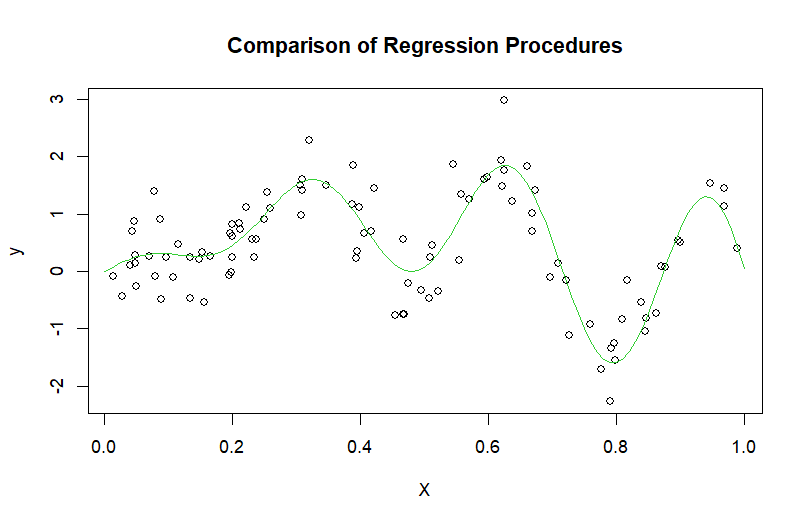
\includegraphics[width=0.95\textwidth]{comparison1.png}
      \newline
      \small True model
  \end{center}
\end{frame}
\begin{frame}{The nonparametric setting}
  \begin{center}
      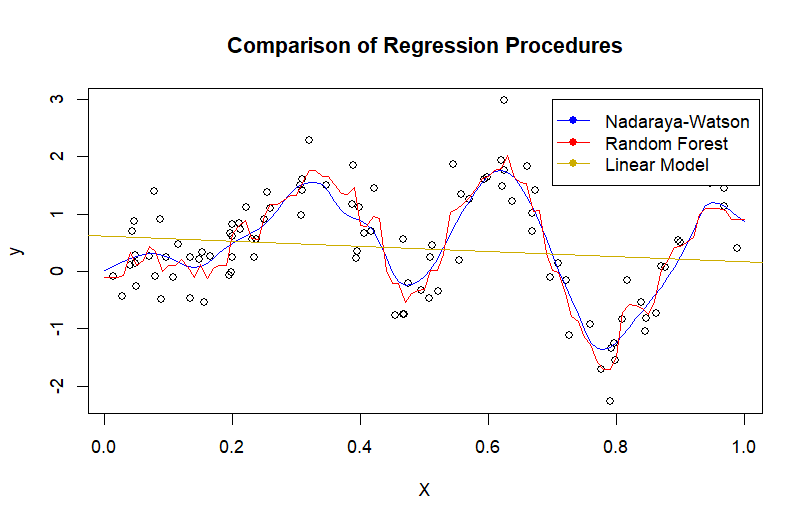
\includegraphics[width=0.95\textwidth]{comparison2.png}
      \newline
      \small Estimators
  \end{center}
\end{frame}

\begin{frame}{The nonparametric setting}
  We will consider the simplified scenario of selecting between two regression procedures, denoted \alert{\(\delta_{1}\)} and \alert{\(\delta_{2}\)}, that yield estimators \alert{\(\hat{f}_{n, 1}\)} and \alert{\(\hat{f}_{n, 2}\)} of the regression function \(f\).

  \textbf{Definition:}
  Let \(L_{n}\) be a loss function. We say \(\delta_{1}\) is \alert{\emph{asymptotically better}} than \(\delta_{2}\) under \(L_{n}\) if, for \(0<\varepsilon<1\), there exists \(c_{\varepsilon}>0\) such that
  \[\prob\set{\Loss{\fhat{n}{2}}\geq (1+c_{\epsilon})\Loss{\fhat{n}{2}} }\geq 1-\varepsilon\]
  for all but finitely many \(n\).

  Given that \(\delta_{1}\) is asymptotically better than \(\delta_{2}\), we say that a selection procedure is \alert{consistent} if it selects \(\delta_{1}\) with probability tending to 1 as \(n\to\infty\).
\end{frame}


\begin{frame}{Nonparametric selection: The hold-out}
    Recall the \alert{hold-out} loss estimator, defined by
  \begin{equation}\label{def:holoss}
      \ho(\fhat{n}{j}) = \sum_{i=n_{1}+1}^{n}\paren{y_{i} - \fhat{n_{1}}{j}(\x_{i})}^{2}\quad\text{for }j=1,2.
  \end{equation}
  We write \(\fho\) to denote the estimator selected by \(\ho\).
  To show the consistency of \(\ho\), we establish two assumptions:  
  \begin{itemize}
    \item We assume the existance of two positive sequences \(\set{A_{n}}_{n\geq1}\) and \(\set{M_{n}}_{n\geq1}\) such that 
    \begin{equation}\label{eq:lpconditions}
      \norm{f-\fhat{n}{j}}_{\infty} = \Op{A_{n}}\quad\text{and}\quad\frac{\norm{f-\fhat{n}{j}}_{4}}{\norm{f-\fhat{n}{j}}_{2}} = \op{M_{n}}
    \end{equation}
    \item We will assume that one of \(\delta_{1}\) and \(\delta_{2}\) is asymptotically better than the other.
    
  \end{itemize}
\end{frame}

\begin{frame}{Nonparametric selection: The hold-out}
\begin{block}{Theorem (\cite{yang_2007})}
    Suppose that the conditions established above hold. Suppose, furthermore, that
    \begin{enumerate}
        \item \(n_{1}\to\infty\) as \(n\to\infty\)
        \item \(n_{2}\to\infty\) as \(n\to\infty\)
        \item \(n_{2}M_{n_{1}}^{-4} \to \infty\) as \(n\to\infty\)
        \item \(\sqrt{n_{2}}\max(p_{n_{1}}, q_{n_{1}})/\paren{1+A_{n_{1}}}\to\infty \) as \(n\to\infty\)
    \end{enumerate}
    Then, the hold-out CV procedure is consistent.
\end{block}
\end{frame}

\begin{frame}{Nonparametric selection: The hold-out}
  \begin{example}
    Suppose that \(\fhat{n}{1}\) and \(\fhat{n}{2}\) are two nonparametric estimators with rates of convergence \(p_{n}=O\paren{n^{-4/9}}\) and \(q_{n}=O\paren{n^{-1/3}}\), respectively. Suppose that (\ref{eq:lpconditions}) is satisfied with \(A_{n} = O(1)\) and \(M_{n}=O(1)\). If we choose splits such that \(n_{1}\to\infty\) and \(n_{2}\to\infty\) as \(n\to\infty\), then \(n_{2}M_{n_{1}}^{-4}\) is clearly satisfied and 
    \[\frac{\sqrt{n_{2}}\max(p_{n_{1}}, q_{n_{1}})}{1+A_{n_{1}}} \geq \frac{n_{2}^{1/2}}{n_{1}^{1/3}}\to\infty \]
    is satisfied if \(n_{1}=o\paren{n_{2}^{3/2}}\). In other words, it is possible for the estimation size \(n_{1}\) to be dominating.
  \end{example}
\end{frame}

\begin{frame}{Nonparametric selection: The hold-out}
  \begin{example}
    On the other hand, if at least one of \(\fhat{n}{1}\) and \(\fhat{n}{2}\) has a parametric rate of convergence \(O(n^{-1/2})\), then
    \[\sqrt{n_{2}}\max(p_{n_{1}},q_{n_{1}})\geq \paren{\frac{n_{2}}{n_{1}}}^{1/2}\to\infty\]
    is satisfied whenever \(n_{2}/n_{1}\to\infty\). This agrees with the conclusion from Section~\ref{sec:lm}, in which we showed that cross-validation is often consistent if the validation size dominates.
  \end{example}
\end{frame}

\begin{frame}{Nonparametric selection: Voting CV}
   We introduce the \alert{majority-vote cross-validation}: For each permutation \(i\mapsto\pi(i)\) of the data, we compute the estimators \(\fhat{n_{1}}{1}\) and \(\fhat{n_{1}}{2}\) using the first \(n_{1}\) data points,
  \[\data^{E_{1}} = \set{\paren{y_{\pi(1)}, \x_{\pi(1)}}, \ldots,\paren{y_{\pi(n_1)}, \x_{\pi(n_1)}}},\]
  as the training sample and the remaining \(n_{2}=n-n_{1}\) elements as the validation sample. We then find the estimator that minimizes the hold-out loss
  \[\hat{R}_{\pi}(\fhat{n}{j}) = \sum_{i=n_{1}+1}^{n}\paren{y_{\pi(i)} - \fhat{n_{1}}{j}\paren{\x_{\pi(i)}}}^{2}\qquad \text{for }j=1,2.\]
\end{frame}

\begin{frame}{Nonparametric selection: Voting CV}
  The chosen estimator is the one favored by the majority of the permutations.
  Let 
  \[\tau_{\pi} = \ind{\hat{R}_{\pi}(\fhat{n}{1}) \leq \hat{R}_{\pi}(\fhat{n}{2})}\]
  The majority-vote estimator selection rule is as follows:
  \[\hat{f}_{n} = \begin{cases}
      \fhat{n}{1} &\text{if }\sum_{\pi\in\Pi}\tau_{\pi} \geq {n!}/{2},\\[2mm]
      \fhat{n}{2} &\text{otherwise,}
  \end{cases}\]
  where \(\Pi\) denotes the set of all permutations of \([n]\).
\end{frame}

\begin{frame}{Nonparametric selection: Voting CV}
  \begin{block}{Theorem (\cite{yang_2007})}
    Under the conditions of the previous Theorem and the condition that the data is iid, the majority-vote cross-validation method is consistent.
  \end{block}

  \textit{Proof: }
  Suppose that \(\delta_{1}\) is asymptotically better than \(\delta_{2}\). For \(\pi\in \Pi\), we have that
  \[\prob\set{\hat{L}_{\pi}\paren{\fhat{n}{1}} \leq \hat{L}_{\pi}\paren{\fhat{n_{1}}{2}}} = \Ep{\tau_{\pi}} \stackrel{(*)}{=} \Ep{\frac{1}{n!}\sum_{\pi\in\Pi}\tau_{\pi}}.\]
  The equality at \((*)\) follows from the fact that the data are iid, hence exchangeable, and thus the \(\tau_\pi\) are identically distributed. By the previous theorem, the right-hand side converges to 1 as \(n\to\infty\). Since the average \(1/n! \sum_{\pi}\tau_{\pi}\) is almost surely at most 1, it follows that \(1/n! \sum_{\pi}\tau_{\pi} \to 1\) in probability, and the majority-vote cross-validation method is consistent.\qed{}
\end{frame}

\begin{frame}{Nonparametric selection: Voting CV}
  \textbf{Remark 1: } The proof does not require using the entire set \(\Pi\) of permutations for the majority vote. 
  
  \textbf{Remark 2: }These conditions are not merely sufficient but necessary
  
  \(\implies \) The number of splits does not affect consistency. In other words, multiple splits in cross-validation cannot rescue an inconsistent single-split procedure.
\end{frame}

\begin{frame}{Nonparametric selection: Key points}
  \begin{itemize}
    \item Key distinction: In nonparametric settings, training set dominance is acceptable for consistency, unlike the parametric case.
    \item Cross-validation is effective for comparing estimators with different convergence rates.
    \item Both single-split and voting methods can yield consistent selection under suitable norm conditions.
    \item Leave-one-out CV is generally inadequate due to its small validation size.
    \item Averaging approaches may retain more data and are likely asymptotically equivalent to voting methods (\cite{yang_2007}).
  \end{itemize}
\end{frame}

\section{Conclusion}
\begin{frame}{Conclusion: Cross-Validation for Model Selection}
    \begin{itemize}
      \item \textbf{Linear Models:}
        \begin{itemize}
          \item For consistent model selection, validation set size must dominate: $\frac{n_2}{n_1} \to \infty$ as $n \to \infty$
          \item The leave-one-out CV is effective only when at most one correct model with fixed dimension exists.
          \item The delete-\(d\) method performs well when fixed-dimension correct models exist.
        \end{itemize}
      \item \textbf{Nonparametric Setting:}
        \begin{itemize}
          \item Training set dominance can be acceptable for consistency.
          \item Single-split and voting methods can both yield consistent selection under suitable norm conditions.
          \item Leave-one-out CV remains inadequate due to minimal validation size
          \item Multiple splits alone cannot rescue an inconsistent single-split procedure
        \end{itemize}
    \end{itemize}
\end{frame}

\begin{frame}
    \frametitle{Conclusion}
    \textbf{Practical Implications:}
        \begin{itemize}
            \item Though computationally costly, cross-validation may be worth using.
            \item The result on the majority-vote approach suggests that few splits can still yield consistency (i.e., \(k\)-fold remains useful).
        \end{itemize}
    \textbf{Remain to be addressed:}
        \begin{itemize}
            \item Split ratios.
            \item Number of splits.
            \item Voting versus averaging.
        \end{itemize}
\end{frame}

\begin{frame}
    \frametitle{Questions?}

    \begin{itemize}
        \item How do you use cross-validation?
        \item What behaviors have you observed in practice?
    \end{itemize}

    

\end{frame}

\end{document}
